% Name: Trace
% Description: A morphism with its output bent around to its input: the categorical trace, a closed loop.
% Tags: trace, loop, pivotal category

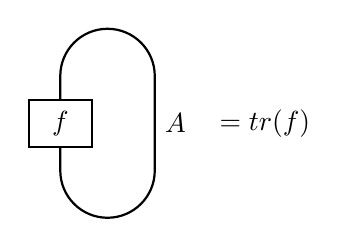
\begin{tikzpicture}[thick, baseline=(current bounding box.center)]
  \draw (0,-0.6) -- (0,0.6) arc[start angle=180, end angle=0, radius=0.6]
    -- (1.2,-0.6) arc[start angle=360, end angle=180, radius=0.6];
  \node[draw, fill=white, minimum width=8mm, minimum height=6mm] at (0,0) {$f$};
  \node[right] at (1.2,0) {$A$};
  \node at (2.6,0) {$= \operatorname{tr}(f)$};
\end{tikzpicture}
